\documentclass[10pt]{ctexart}

\usepackage{tikz}
\usepackage{verbatim}
\usepackage{amsmath}
\usepackage{graphicx}
\usepackage{float}

\title{一元二次方程在实数域上的求解}
\author{作者姓名: 唐浩 \\ 作者专业学号: 信息与计算科学 3200102118}

\begin{document}

\maketitle

\section{简介}
一元二次方程,字面意思来看,便是只有一个未知数(元),且未知数最高次数为 2 的一个整式方程。其一般形式为 $ax^2 + bx = 0 (a \ne 0)$, 称 $ax^2$ 为二次项,a 为二次项次数; bx 为一次项, b 为一次项系数; c 为常数项。

求解一元二次方程的解,便是求使得一元二次方程左右两边相等的未知数 x 的值,该解也叫做一元二次方程的根(root)。

\section{求解}
求一元二次方程的根的过程便称作求解一元二次方程,其解法众多,接下来我们介绍其中一种解法——— 判别式法:称式子 $b^2 - 4ac$ 为 $ax^2 + bx + c = 0$ 根的判别式,记做 $\varDelta$。$\varDelta$ 有三种情形:1) < 0, 2) = 0, 3) > 0。 下面我们就这三种情况分别进行讨论。哦对了,在此之前将方程进行配方,得

\[
(x + b/2a)^2 = (b^2 - 4ac)/(4a^2)
\]

\subsection{当$\varDelta < 0$}

若$\varDelta < 0$,则 $(x + b/2a)^2 < 0$,显然,x 在实数域上取值时,这个解不存在,即方程无实数根。

\subsection{当$\varDelta = 0$}

若$\varDelta = 0$,则 $(x + b/2a)^2 = 0$,显然,此时的 $x = \frac{-b}{2a}$。

\subsection{当$\varDelta > 0$}

若$\varDelta > 0$,则 $(x + b/2a)^2 > 0$,显然,此时方程有两个不同的根,分别为:

\[
x_1 = \frac{-b+\sqrt{\varDelta}}{2a} \quad  x_2 = \frac{-b-\sqrt{\varDelta}}{2a}
\]

具体的算法流程图如下:

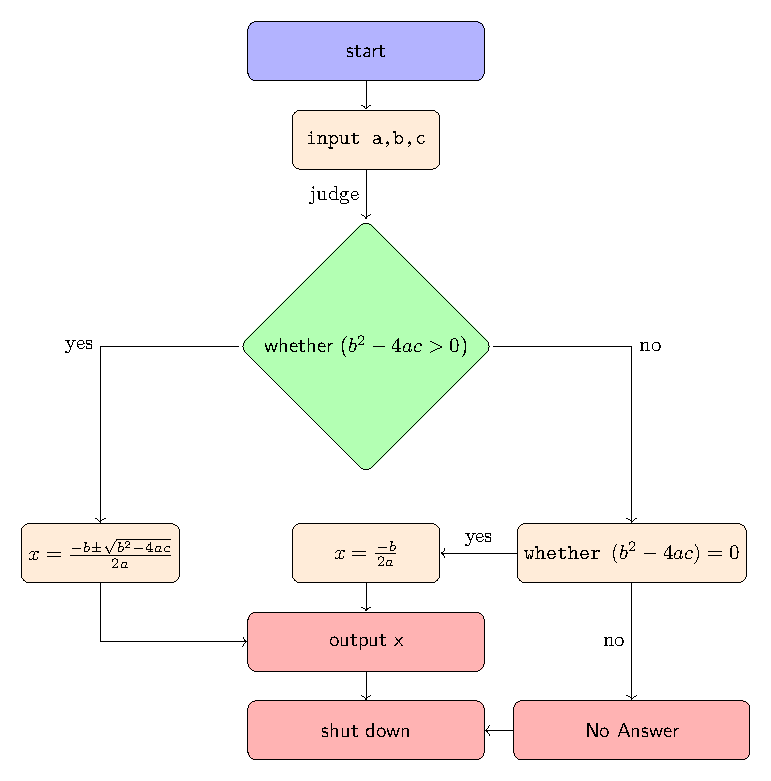
\includegraphics[scale=0.75]{report_tikz.pdf}

\section{总结}
综上所述,当 $\varDelta > 0$ 时,方程有两个不等的实数根;

当 $\varDelta = 0$ 时,方程有两个相等的实数根;

当 $\varDelta < 0$ 时,方程无实数根。

当 $\varDelta \ge 0$ 时,方程的实数根可写为 $x = \frac{-b \pm \sqrt{\varDelta}}{2a}$ 的形式,这个式子叫做一元二次方程的求根公式。

以下给出一个简单的图例:

\begin{figure}[H]
  \centering
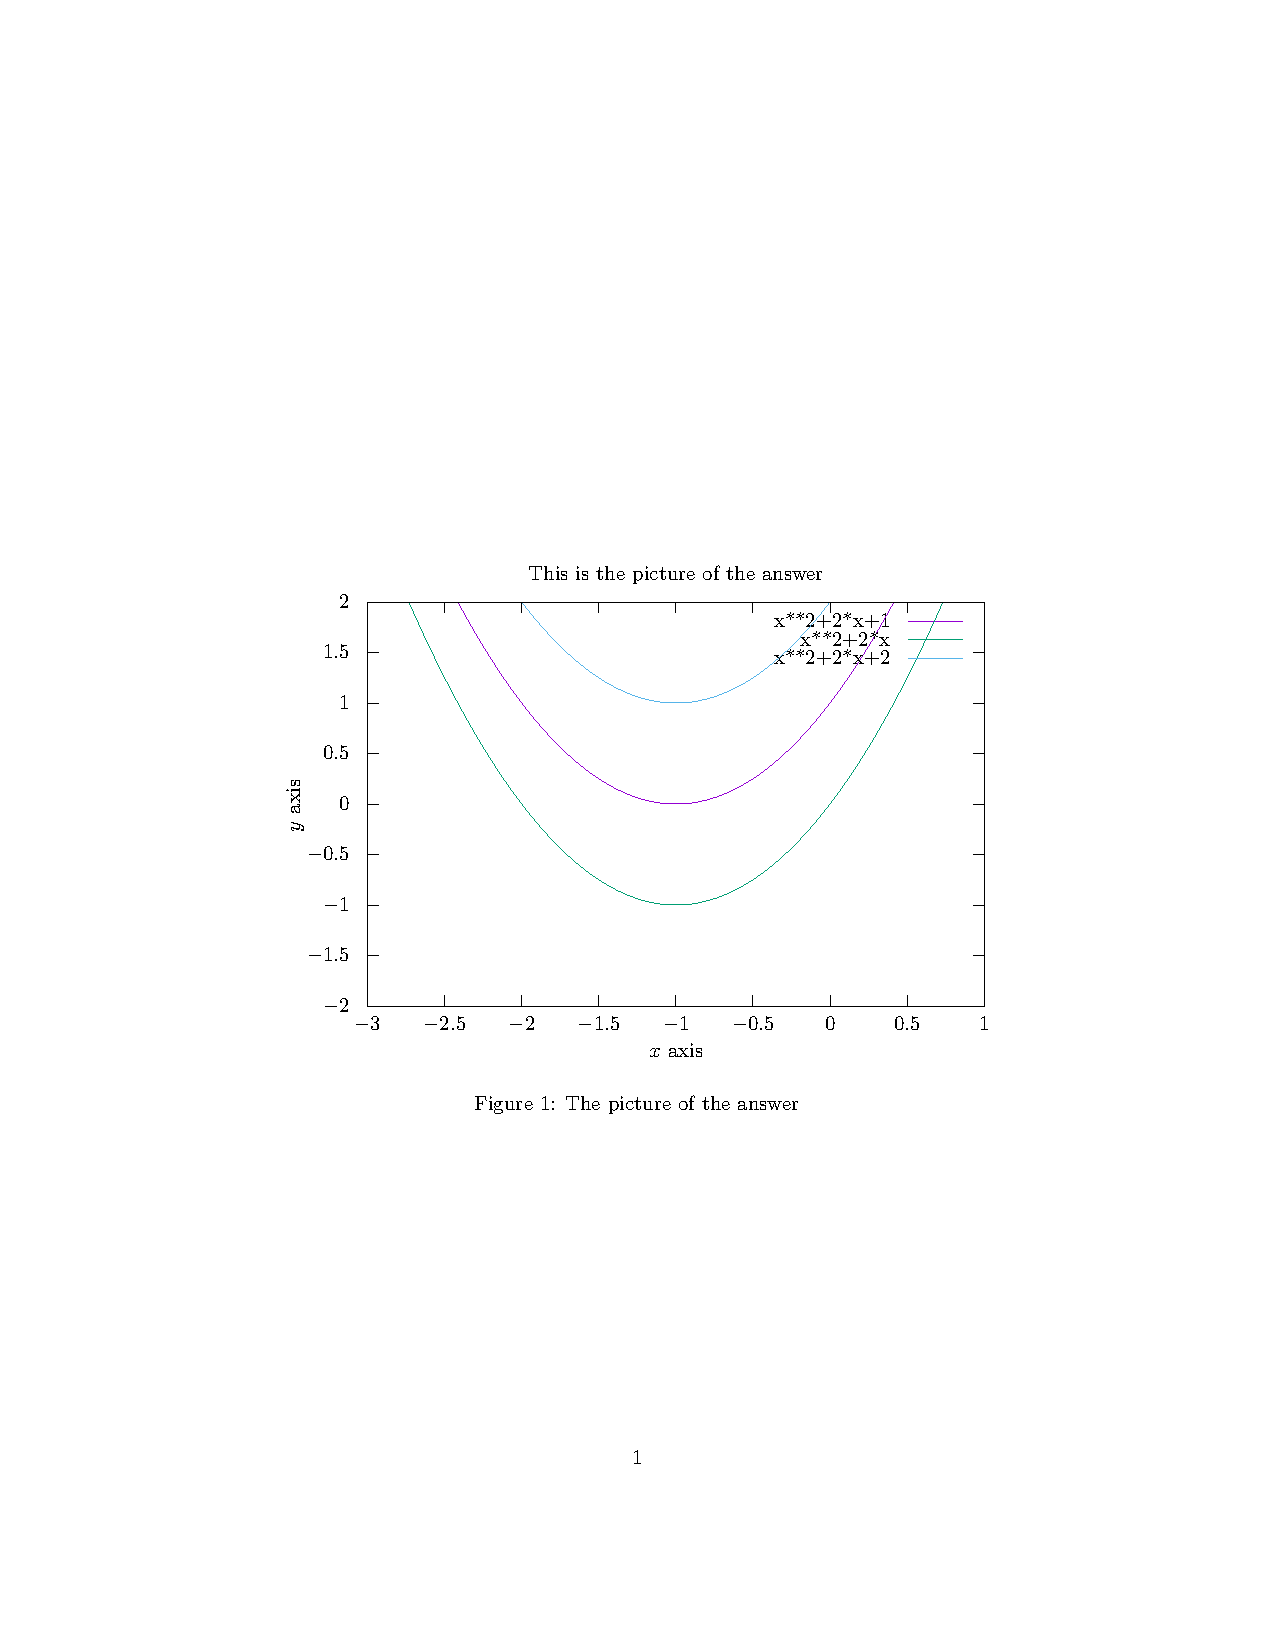
\includegraphics[scale=0.75]{re.pdf}
\end{figure}

\end{document}
